\section{Implementation}
\label{section:implementation}
\subsection{Mobile Player}
In this section the mobile player \gls{prefab} will be discussed. 
\gls{see} is supported on multiple platforms and with each platform having different requirements each platform needs to be divided.
Therefore, each platform gets its own player \gls{prefab}.
The mobile player prefab for the \gls{android} version of \gls{see} can be seen in figure \ref{fig:prefab}.

\begin{figure}[htb]
    \centering
    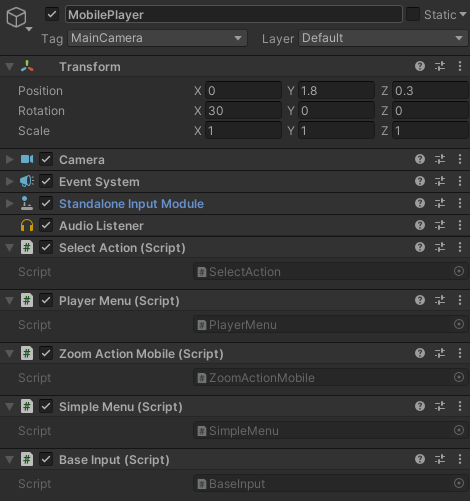
\includegraphics[width=0.8\textwidth]{Implementation/img/mobile_player.png}
    \caption{The mobile player \gls{prefab}}\label{fig:prefab}
\end{figure}

The \gls{prefab} consists of the basic parts provided by \gls{unity} \textit{Camera}, \textit{Event System}, \textit{Standalone Input Module} and \textit{Audio Listener}.
In addition to that the following custom scripts were added.
There is the \textit{SelectAction} and the \textit{ZoomActionMobile} script, which will both be discussed in section \ref{sec:player_actions}, and then there is the \textit{PLayerMenu} script, which creates the right menu based on the player type.
In this case the player type will be \enquote{mobile player} and the menu created (here \textit{SimpleMenu}) will be discussed in section \ref{sec:menu}.

\subsection{Player Movement}
After having creating a player, the player also has to be able to move.
Therefore, the \textit{MobilePlayerMovement} script got added.
The script handles the input by the joysticks seen in figure \ref{fig:joystick}.
To fulfill [R2.1] the player will be moved by using the left joystick and the player's perspective will be handled by the right joystick.

\begin{figure}[htb]
    \centering
    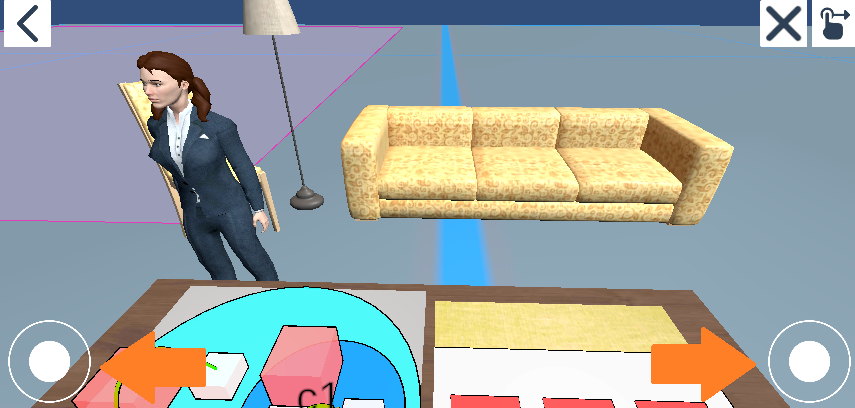
\includegraphics[width=1\textwidth]{Implementation/img/joysticks.png}
    \caption{The joysticks are for moving in the virtual room. The left joystick is for moving the player and the right one is for moving the player's perspective.}\label{fig:joystick}
\end{figure}

For the joystick \glspl{prefab} the \textit{Joystick Pack}\footnote{https://assetstore.unity.com/packages/tools/input-management/joystick-pack-107631\#description (last visited: 17.06.22, 15:21)} \gls{asset} is used.
It contains the design and basic logic for the joysticks.
A joystick returns a horizontal and a vertical value depending on how far the joystick is dragged into a direction.
The left joystick data can then be transformed into player movement as follows:
\begin{enumerate}
    \item Get the horizontal and vertical values from the joysticks
    \item Transform the values into a 3D vector
    \item Combine the values into a velocity vector
    \item Normalize the velocity vector for a smooth transition
    \item Transmit the velocity vector to the player position value
\end{enumerate}

The data of the right joystick shall move the player's perspective, which is implemented as a \gls{unity} camera.
The camera has a pitch angle and a yaw angle as illustrated in figure \ref{fig:camera}.
The angles of the camera will be adjusted with the input from the right joystick. 
For the angles of the player's perspective there is a range from 0° to 360° after reaching an end of this range the value will be transformed to the other end of the range.
In other words if the angle grows higher than 306° it starts an 0° again and if it gets lower than 0° it can go further down from 360°.
That way the player's perspective can move a full rotation.
\begin{figure}[htb]
    \centering
    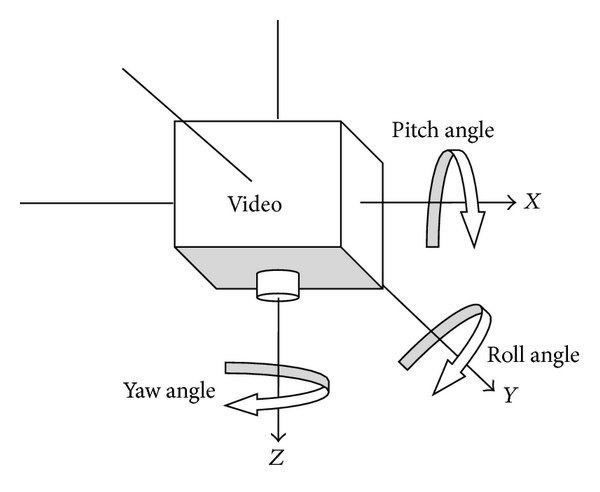
\includegraphics[width=1\textwidth]{Implementation/img/pitch_yaw.jpg}
    \caption{The angles of a camera by \cite{Zhang2014}}\label{fig:camera}
\end{figure}

\subsection{Mobile Menu}
\label{sec:menu}

The mobile menu is essential for the implementation since the input methods of a smartphone in an everyday usage are limited.
The desktop version uses many \glspl{shortcut}, which cannot be used in the mobile version.
These \glspl{shortcut} will replaced with buttons in the menu to fulfill requirement [R2.2].

\begin{figure}[htb]
    \centering
    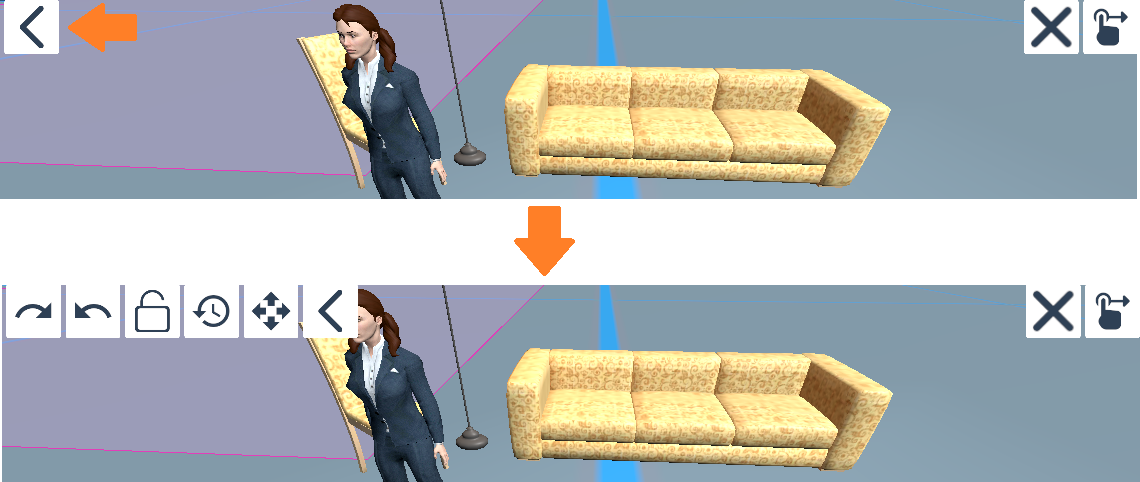
\includegraphics[width=1\textwidth]{Implementation/img/quickmenu.png}
    \caption{The \textit{quickbar} on the left top side of the mobile device. Pressing the button with an orange marked arrow will expand the menu.}\label{fig:quickmenu}
\end{figure}

The menu will be divided into to parts.
The first part, that was named \textit{quickbar} in section \ref{sec:interface}, will be responsible for all interactions that need to be available at all times.
The implemented \textit{quickbar} can be seen in figure \ref{fig:quickmenu}.
By pressing the button on the right end of the \textit{quickbar} the menu can be expanded and minimized to safe screen space when not needed.

The other part of the menu can be seen in figure \ref{fig:interaction_menu}.
The menu is placed on the right side of the screen, and it contains all the player interactions.
This part of the menu is slightly more complex since the selected button moves to the top, while the other buttons shall remain their initial order.

\begin{figure}[htb]
    \centering
    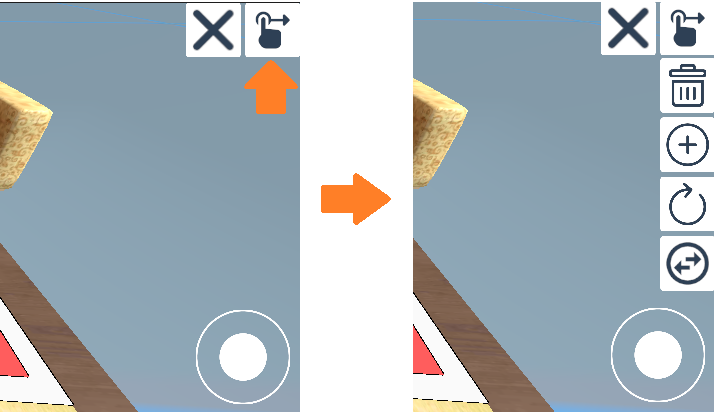
\includegraphics[width=1\textwidth]{Implementation/img/menu.png}
    \caption{The player interaction menu on the right top side of the mobile device. The button on the top right side indicate the active interaction mode. Pressing the same button also expands the menu.}\label{fig:interaction_menu}
\end{figure}

The implementation of the menu on the right is done in the following steps:
\begin{enumerate}
    \item All main buttons get an index
    \item When a button on the far right side gets clicked the index gets saved
    \item The button group with the selected index get shown on the top right side
    \item All other buttons get disabled
    \item By clicking the button on the top right again the other main buttons get reactivated 
    \item The order is as follows: selected index → index in ascending order
\end{enumerate} 
This way the selected interaction mode will always be in the top right corner, while the other buttons remain the same order.

\subsection{Player Actions}
\label{sec:player_actions}

One essential part of the implementation are the player actions. 
Almost all interactions a user can make in \gls{see} differ from the interactions in the desktop version.
In the following the implementation of all mobile player actions will be shortly discussed.

\subsubsection{Zooming}
To fulfill requirement [R2.3] zooming needs to be implemented.
The interaction of zooming in or out of a \gls{city} can be fundamental when working with a large \gls{city} because \glspl{node} become small and especially on a small mobile screen it becomes impossible to interact with those nodes via touch input. 
Therefore, the user has to zoom in to properly interact with the desired node.

Luckily the general zooming function is already implemented in \gls{see}.
The zooming method- requires a center point and a scale of how far the \gls{city} shall be zoomed in or out.
Zooming on a touchscreen will be done by dragging two fingers either towards or away from each other as visualized in figure \ref{fig:zooming}.

\begin{figure}[htb]
    \centering
    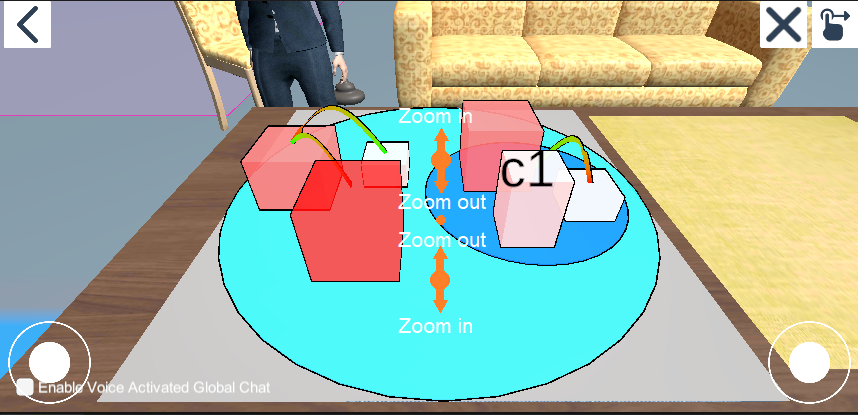
\includegraphics[width=1\textwidth]{Implementation/img/zoom.png}
    \caption{Dragging the two touch points towards each other will zoom out and dragging them away from each other will zoom in.}\label{fig:zooming}
\end{figure}

The implementation of the zooming interaction in done in the following steps: 
\begin{enumerate}
    \item Check if there are two touch inputs on the same \gls{city}. If both inputs are not on the same city zooming is not wanted and will not be activated.
    \item Compute the center of the two touch inputs
    \item Pass the center and dragging range of the two inputs to the zooming function
\end{enumerate}

Note that the direction of zooming has been inverted in the version used for the evaluation in chapter \ref{section:evaluation}.
This is because of the heavy demand by the subjects to invert the direction of zooming since it feel odd.

\subsubsection{Selecting and Deleting}
The interactions of selecting and deleting a \gls{node} or \gls{plane} are quite similar because the user selects or deletes an object by touching it.
The object get determined by a ray cast from the center of the touch position as discussed in section \ref{sec:ray}.

Since the selecting mode is always enabled except when the delete mode is active, the select button really does nothing except ensuring that no other interaction mode is active.
Keeping the selected objects active makes sense for the mobile version because the user cannot hover with a mouse to see the object names.
Therefore, the selection will be kept and not discarded by selecting a different object as in the desktop version.
The deselect button call the already implemented \textit{UnselectAll} method that empties a list of selected items.

To delete interaction works as already mentioned just like in the desktop version. 
The only difference is the type of input. 
Other than in the desktop version the mobile version only supports single deletions and not the deletion of multiple objects at once.
This is due to the limited space for the interactions menu and the results from a multi deletion can also be achieved with the single delete interaction.

The discussed implementation fulfills requirements [R3] and [R4].
\subsubsection{Node Interactions}
The node interactions consist of four types.
The active interaction is always highlighted in green as seen in figure \ref{fig:node}
\begin{figure}[htb]
    \centering
    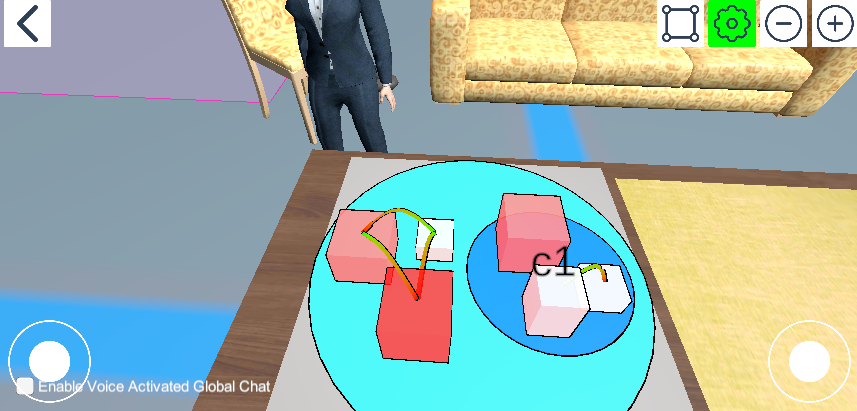
\includegraphics[width=1\textwidth]{Implementation/img/node.png}
    \caption{The node interactions menu. The active node interaction has a green button}\label{fig:node}
\end{figure}

The circled plus button stands for adding a \gls{node}.
Adding \glspl{node} is implemented in the following steps:
\begin{enumerate}
    \item Check if the device is an \gls{android} with a preprocessor tag
    \item Check if there is exactly on touch input
    \item Cast a ray and check if the collided object is of the type \enquote{Node} (\gls{see} does not distinguish between \gls{plane} and \gls{node} as a type)
    \item Create a \gls{node} ad that position with the already implemented \textit{AddChild} method of the class \textit{GameNodeAdder}
\end{enumerate}

The circled minus button is for adding an \gls{edge}.
The implementation is quite similar to the one for adding \glspl{node}.
In this case however the first and second \gls{gameObject} of type \enquote{\gls{node}} will be saved.
After there are two \glspl{gameObject} an \gls{edge} between those objects will be created.

Next in line is the gear button, which can be used for editing \glspl{node}.
The implementation here is almost the same as for the desktop version.
A \gls{node} or a \gls{plane} can be selected by touch and a window will open.
In that window attributes like the name can be changed.
Different from the desktop version is that a virtual keyboard will pop up to let the user type in a new name for example.

Last but not least there is the interaction of scaling a node left.
The implementation here was largely adopted from the desktop version, except again the input type is via touch.
In addition to that the dots that can be selected and dragged are larger in the mobile version (see figure \ref{fig:scale}) because otherwise it would be hard to hit them with a touch input.

\begin{figure}[htb]
    \centering
    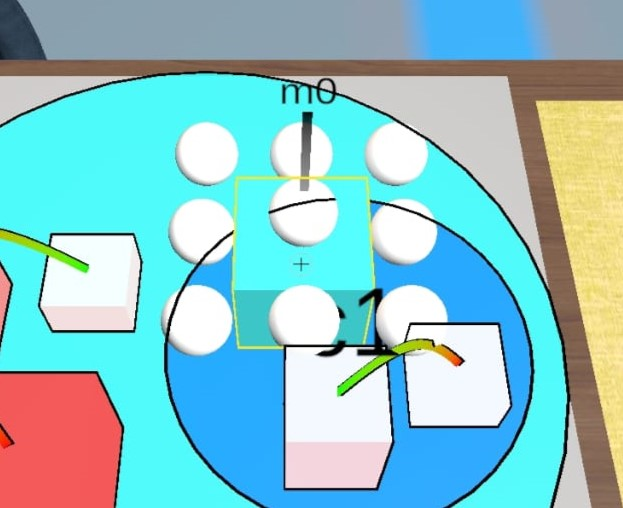
\includegraphics[width=0.7\textwidth]{Implementation/img/scale.jpeg}
    \caption{The node interactions menu. The active node interaction has a green button}\label{fig:scale}
\end{figure}

The listed implementations of the node interactions fulfill the requirements of [R5].

\subsubsection{Rotating}
[R6]

\begin{figure}[htb]
    \centering
    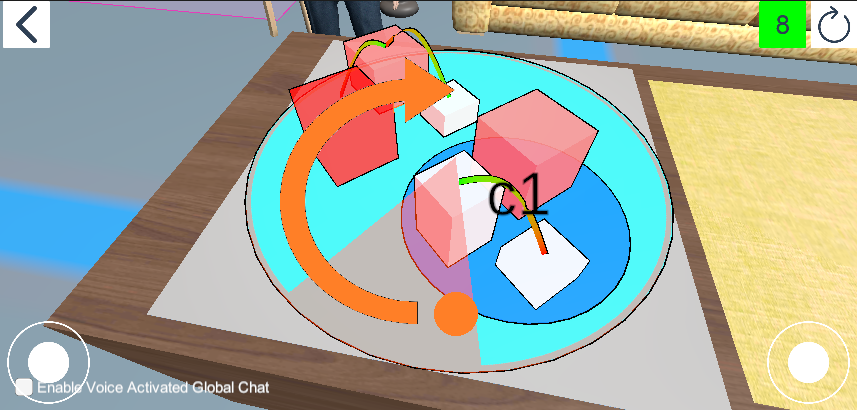
\includegraphics[width=1\textwidth]{Implementation/img/rotate.png}
    \caption{The \gls{city} can be rotated by for example touching the screen on the orange dot and dragging from there like the arrow indicates.}\label{fig:rotate}
\end{figure}
\subsubsection{Moving}
[R7]

\begin{figure}[htb]
    \centering
    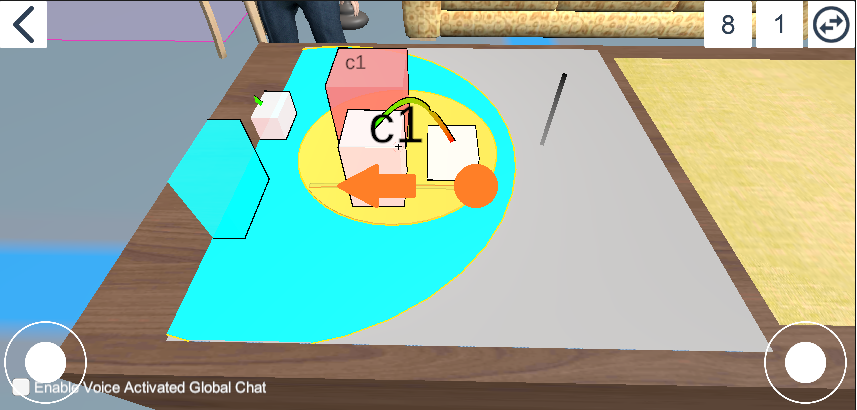
\includegraphics[width=1\textwidth]{Implementation/img/move.png}
    \caption{The \gls{city} can be moved by touching and dragging it to a desired direction.}\label{fig:left}
\end{figure}
\subsection{Android Build Requirements}
[R1]
\subsubsection{Preprocessor Tags}
\subsubsection{Restructure}
\subsubsection{File Loading}